\newcommand{\FigMuecCreation}{
\begin{figure}[bt]
\centering 
%\fbox{
%\input{figs/feynman/mu_to_e_gamma_via_SM-Wgamma.tex}
\subfloat[][\figlabel{muec:underlying}Underlying Process]{%
\includegraphics[width=0.32\textwidth,trim=-0.6cm 0 -0.6cm 0,clip]{figs/feynman/pdfs/mu_e_conversion.pdf}}\hspace{0.01\textwidth}%
\subfloat[][\figlabel{muec:atomSketch}Conversion from Ground State]{%
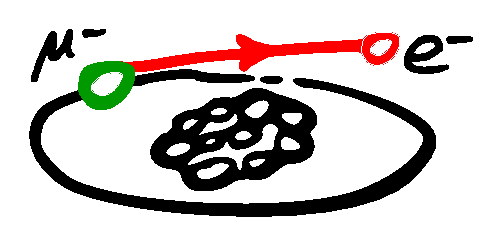
\includegraphics[width=0.30\textwidth]{figs/mueconv/MuEConversion-atom-sketch.pdf}}\hspace{0.01\textwidth}%
\subfloat[][\figlabel{muec:beamOnTgt}Muon Beam Stopped in Target]
\caption{\figlabel{muec:creation}
The underlying \mueconv process \protect\subref{fig:muec:underlying} occurs from the ground state of a muonic atom~\protect\subref{fig:muec:atomSketch}.
To produce the muonic atoms a beam of muons has to be stopped in a target~\protect\subref{fig:muec:beamOnTgt}.
}
%\footnote{though the author has failed to reproduce the stereoscopic effect with his own eyes}
\end{figure}
}


\chapter{Muon-to-Electron Conversion and the Muonic Atom}
\sectlabel{theory:atomicMuon}
Muon-to-electron conversion is the spontaneous decay of a muon to an electron within the Coulomb potential of an atomic nucleus and without the emission of neutrinos.
It proceeds according to the formula:
\begin{equation}
\mu^{-}+N(A,Z) \rightarrow e^{-}+N(A,Z)
\end{equation}

In general, the nucleus involved can be excited under \mueconv, although all experimental searches to date have required that the nucleus be left unchanged.
This constraint has two effects: firstly, coherent terms in the \mueconv cross section dominate, since the interaction will largely take place with the whole nucleus.
Being coherent, the rate of \mueconv will, in general, grow more quickly as a function of the atomic mass or number (though exactly which of these determines the rate is itself model dependent).
Secondly, the constraint of an unchanged nucleus means that all the free energy of the initial muon has to go into the kinetic energy of the electron and the recoil of the nucleus.
Since the initial system is at rest, and as a two body decay, the energy of the outgoing electron is fixed:
\begin{equation}
E_e=M_\mu-E_{\mu,\mathrm{binding}}-E_\mathrm{recoil}
\end{equation}
where $M_\mu=$105.66~MeV/c$^2$ is the muon mass, $E_{\mu,\mathrm{binding}}$ the
binding energy of the muon in the ground state of the muonic atom, and
$E_\mathrm{recoil}$ is the kinetic energy of the recoiling nucleus.
In the aluminium target used for COMET (see section \sect{stop-tgt}) the electron energy is $E_e=104.97$~MeV.
The simplicity and model independence of the signal---a single, monoenergetic electron---makes the process experimentally very attractive.

\FigMuecCreation
The various scales involved in a search for \mueconv are illustrated in \fig{muec:creation}.
To observe \mueconv, a muonic atomic is formed with the muon in the ground state.
An interaction between the muon and the nucleus causes Lepton Flavour Violation and producing an electron.
In order to form the muonic atoms, a beam of negative muons is brought to stop in a target and the resulting electrons, if \mueconv takes place, then detected.

When muons in the beam enter the target they will initially lose energy predominantly through ionisation.
Once they reach energies of around a few keV they become atomically bound to the Coulomb potential of the nucleus.
From here, on the order of 100~fs, these muons will undergo Auger and radiative transitions to the ground state.
The X-rays emitted during this electromagnetic cascade have well defined energies and intensities and can therefore be detected as a means to evaluate the number of muons stopped in the target.
\Fig{muec:alXrays} shows the most intense transition peak, $2p-1s$ in the X-ray spectrum for muonic aluminium, and the muonic magnesium lines that occur with similar energies.

\FigMuonicXrays
From the ground state there are two processes that can occur to the bound muon in the \ac{SM}:
\acf{DIO} and nuclear capture.
\ac{DIO} is the normal decay of a muon with neutrino emission, although the spectrum of the emitted electron is modified compared to the free muon decay due to the presence of the nucleus.
Nuclear capture of the muon occurs when the muon is absorbed into the nucleus decreasing the atomic number by a single unit, in analogue to nuclear electron capture or inverse beta decay.
A single muon-neutrino is emitted as well as various possible gamma-rays and hadrons, since the daughter nucleus is often unstable.

Both of these are important in \mueconv searches, since they impose various experimental constraints.
Furthermore, these two processes determine the lifetime of the bound muon, which is not the same as the free muon.
In the case of decay, being bound to the nucleus reduces the available energy, therefore reducing the available phase-space for the resultant electron and neutrinos. 
In addition, a time-dilation effect occurs since the bound muon is never truly at rest. 
As a result, the partial lifetime of muon decay increases in the bound muon system compared to the free muon, and this increase grows with the atomic number as the muon binds more tightly to the nucleus.
However, whilst the rate of decay decreases with atomic number the rate of muon capture increases.
This occurs, firstly, because there are more protons against which to capture and, secondly, because the overlap between the muon wavefunction and the nucleus increases.
For atomic numbers larger than $Z=30$ this effect begins to saturate since the muon wavefunction becomes contained almost completely within the nucleus.
Whilst for light elements, up to around $Z=12$, the decay process is more frequent, for the rest of the periodic table the capture process dominates.
For an aluminium target, the two processes are comparitively similar, with branching ratios of 61 and 39\% for capture and decay respectively, giving the muon a lifetime of 864~ns\footnote{
This is very important to the COMET experiment and so we revisit this aspect in the next chapter.%
}~\cite{Measday2007Comparison}.

Since the muon is 200~times heavier than the electron, the muon wavefunction feels the effect of the nucleus a lot more, creating some theoretical uncertainty on the initial muon wavefunction.
Rather than the full branching ratio, typically \mueconv experiments discuss the conversion rate, which is given by:
\begin{equation}
\mathcal{C.R.}=\frac{\Gamma\left(\mathrm{\mueconv}\right)}{\Gamma\left(\mathrm{nuclear~capture}\right)}
\end{equation}
which reduces the theoretical uncertainty introduced from the initial wavefunction.
%The key advantage of this definition compared to the full branching ratio is that by normalising to the number of muons that undergo nuclear capture, as opposed to the total number of stopped muons, the theoretical uncertainty due to the initial muon wave-function is reduced since it effects capture and conversion in the same way.

Based on this, one defines the \acf{ses} to be:
\begin{equation}
	\eqlabel{det:ses}
\mathrm{S.E.S}(\muec)=\frac{1}{N_\mu \mathcal{B}_\mathrm{capture} A_{\mu\rightarrow e}}
\end{equation}
where $N_\mu$ is the number of muons stopped, $\mathcal{B}_\mathrm{capture}$ is the branching ratio for muon nuclear capture, and $A_{\mu\rightarrow e}$ is the total acceptance of electrons coming from \mueconv.

\section{Muon Decay in Orbit}
In free muon decay the maximum energy for the outgoing electron occurs when the neutrinos recoil back-to-back with the electron.
In this configuration, exactly half the energy released in the decay is available to the electron, so that the maximum energy of an electron coming from the decay of a free and stationary muon is: $\max(E_{e}^\textrm{free})=m_\mu/2=52.5$~MeV.

The end-point configuration is altered significantly once the muon becomes bound to the nucleus of an atom.
Once bound, the neutrinos can be arranged back-to-back with one another, and thus carry away a negligible amount of energy.
Four-momentum can still be conserved however, since the nucleus of the atom recoils against the electron.  
Given the enormous mass of any nucleus compared to the electron, conservation of momentum is possible for small kinetic energies of the nucleus and thus the maximum electron energy is hugely increased compared to the free decay.
In fact, in the limit where the neutrinos carry away no energy, the kinematic configuration of this decay becomes identical to that of \mueconv, but for the mass of the neutrinos\footnote{
It would be interesting whether precise observations at the DIO end-point would be sensitive to the absolute neutrino masses of the muon and electron neutrinos, $\langle M_{\bar{\nu_{e}}}\rangle+\langle M_{\nu_{\mu}}\rangle$.
The current limits of less than 1~eV mean a direct measurement of the end-point is not realistic, but if the shape of the spectrum contained information then this might be exploitable.
Certainly, massive sterile neutrinos could be searched for as a kink or shoulder at the DIO end-point with sensitivity to masses down to a few MeV.
}, and accordingly: $\max(E_{e}^\textrm{DIO})\simeq{}E_{e}^\textrm{conversion}$.
\FigDecayInOrbitSpectrum

The spectrum of electrons from \ac{DIO} in aluminium is shown in \fig{muec:dio}.
It can be seen how the peak electron energy is close to the free muon decay end-point, and in reality about 99\% of \ac{DIO} electrons will be emitted below 58~MeV.
Whilst the end-point for the spectrum is indeed around 104.97~MeV, it is clear how suppressed this part of the spectrum is---some twenty orders of magnitude less likely than at the peak energy.
Achieving the end-point energy requires radiative connections between the nucleus and either the incoming muon, intermediate $W$-boson, or the outgoing electron; the low value of the neutrino momenta brings about a helicity suppression; and the specific energies of all particles implies a small phase-space volume for the decay products.

Given the enormous suppression at the end-point, \mueconv searches historically described themselves as `background free'.
However, at the projected sensitivities of modern experiments, the \ac{DIO} rate close to the end-point of the spectrum is now at an appreciable level.
Indeed, the next generation of searches (and COMET \phaseI in particular) will be the first to measure the \ac{DIO} spectrum above 90~MeV, itself an important cross-check for the theoretical prediction of muon \ac{DIO}%
\footnote{In addition to neutrino mass and sterile neutrino searches, the precision measurement of the end-point of the DIO spectrum feels like it should be extremely interesting for theoretical physicists given  its connection to things like muon g-2 and the Lamb-shift of muonic hydrogen. The end-point calculation requires radiative corrections, which would likely be sensitive to vacuum corrections in a similar way to these other measurements.  If, at COMET \phaseI, we observe any deviation in this region, even if it does not look like \mueconv, I would be very excited of the additional evidence this might imply for lepton non-universality.  In contrast, if we observe no deviation, might this be translated into limits on New Physics models that explain the other anomalies?}.

\section{Muon Nuclear Capture}
%\begin{easylist}
%# Inverse beta-decay
%# Prompt process of muon-proton -> neutron and neutrino
%# Nucleon clustering means prompt protons also observed (muon-nucleon cluster -> neutrino-neutron-proton)
%# about 50~MeV excitation of the nucleus
%# Emission of various particles during nuclear de-excitation: protons, neutrons, gammas, deuterons, triton, alphas
%# Difficult to predict products and rates theoretically
%# Interest in this process towards the end of the 70s as a means to test nuclear theory but since then interest has waned
%# Lack of experimental measurements for Al($\mu$,X)Mg so needed to measure things: \alcap
%# See appendix for an overview of \alcap
%# Proton emission around 3.5\% of every muon captured
%\end{easylist}
The nuclear capture of negative muons is governed by the equation:
\begin{equation}
\mu^-+N(A,Z)\rightarrow \nu_\mu+N'(A,Z-1)
\end{equation}
and as an incoherent process, one would expect direct capture of the muon against a proton to result in a prompt neutron being produced.
However, prompt protons can also be produced if the capture takes place between a nucleon cluster and the muon.
The typical nuclear excitation from such a process is around 50~MeV, with the remainder of the total incoming energy lost to the outgoing neutrino and nuclear recoil.
Even if prompt neutrons and protons are produced, the remnant nucleus is often left in an excited, unstable state, such that during de-excitation other particles can also be emitted.
These include gamma-rays, deuterons, triton and alpha particles as well as additional neutrons and protons.
\FigMuecMuCapture

From the perspective of a sensitive \mueconv experiment, the emission products following nuclear capture can be dangerous since, in the case of charged particles, they can swamp the detector if left unchecked.
Similarly, neutrons and gamma rays produced by nuclear capture can damage electronics systems if left unchecked.
As such it is important to understand the rates at which these particles are emitted following nuclear capture of the muon.

However, due to the nuclear environment theoretical predictions of the rates and energy distributions of capture products are extremely complex, and experimental measurements are necessary.
Unfortunately, in the case of aluminium---the target choice for \COMET---the existing experimental data is not extensive.
\Fig{muec:mucap} shows a summary of the available literature, where one can see how incomplete the current available data is.
Accordingly, it has been necessary to measure this directly.

The \alcap experiment~\cite{AlcapProposal2012} is a joint effort between COMET and Mu2e tasked with measuring the rate and spectra of particles emitted following muon capture in aluminium.
Three runs have been held at \ac{PSI} from 2013 to 2015, and data analysis is on-going, although preliminary neutron and proton spectra and rates have been achieved.
The measured proton rate is low enough that \COMET does not expect to have to take any precautionary measures to reduce it further.
For more information on \alcap, see appendix~\sect{alcap} and the PhD thesis by Nam Tran~\cite{NamThesis}.

\section{Experiments Searches for \mueconv }
\subsection{\sindrumII: Present Limits}
\FigMuecSindrumII
The \sindrumII experiment operated at the \ac{PSI}, last taking data in 2000.
As well as searching for \muThreeE, they also set the 
current limit on \mueconv, published in 2006 to be $\mathcal{C.R}<$\senseSindrum at 90\% confidence level.
The experiment, shown in \fig{muec:sindrum}, used a gold target sitting in the centre of a cylindrical detector.
Both of these sat coaxially with a solenoidal field allowing for momentum measurements by reconstructing the helical trajectories of the detected electrons.

The dominant backgrounds at \sindrumII were cosmic events and pions in the beam.  
The observed energy distribution (from the main event category) is shown to the right of \fig{muec:sindrum}.  
The single Class 1 event that was observed above the expected \mueconv energy in gold was attributed to a pion in the beam.

\subsection{MECO and MELC}
Towards the end of \sindrumII operation, preparation for experiments that would reach to sensitivities around $10^{-16}$ were made.
The first, MELC~\cite{MELC}, was intended to be built at the Moscow Meson Factory.
The stopping target was to be either aluminium or titanium and, for the first time, the muon beam would be produced from pions captured in a solenoidal magnetic field around the production target.
Partly due to the need to adapt the primary beam at the host facility, MELC was never completed, although some aspects of the experiment had been constructed.

With its cancellation, proponents of the experiment shifted their plans to the United States of America.  
The new proposal, known as MECO, was planned to run at the Berkeley National Lab (BNL), and largely kept the design of the MELC experiment.
With the goal \ac{ses} of \num{2e-17} it was planned that MECO would run in 2004 having been built and comission in the preceding few years~\cite{MECO}
\Fig{mueconv:MECO} shows the MECO experiment's beamline.

Sadly, MECO was never built.  
Plans again shifted, with Fermilab deciding to take on the experiment, now known as Mu2e.
The Mu2e looks a lot like the original MELC design, but shares a lot of common features with the COMET experiment, on which we shall focus from here on.
